% Mora SP Cup 2026 -- Team Voxel
% Preliminary-round report. Compiles on Overleaf with pdfLaTeX.
% Formatting is a disqualification surface: 12pt, 1in margins, no cover page, <=5 pages.
%
% ---------------------------------------------------------------------------
% PAGE COUNT: estimated ~4.8 of the 5 allowed, from a word/figure/table budget --
% no LaTeX engine was available locally to confirm it. CHECK THE PAGE COUNT on
% Overleaf before submitting. If it overflows, apply these in order; each is a
% one-line change and none removes content the brief explicitly asks for:
%   1. Fig. 3 (crops):    width 0.92 -> 0.75\textwidth             (saves ~0.05 p)
%   2. Fig. 1 (dataset):  width 0.49 -> 0.42\textwidth on both     (saves ~0.08 p)
%   3. Table 3: drop the "SCUNet zero-shot" and "Training from scratch" rows,
%      both of which are also argued in the text of section 4  (saves ~0.06 p)
%   4. Last resort: add `twocolumn` to \documentclass. Still 12pt with 1in
%      margins so it stays compliant, and roughly halves the page count -- but
%      the three wide tables then need \begin{table*} to span both columns.
% Do NOT cut section 2 (dataset observations) or section 6 (validation
% strategy): both are explicitly required by the brief.
% ---------------------------------------------------------------------------
\documentclass[12pt,a4paper]{article}
\usepackage[margin=1in]{geometry}
\usepackage{graphicx,booktabs,amsmath,microtype,caption,subcaption}
\usepackage[table]{xcolor}
\usepackage{tikz}
\usetikzlibrary{arrows.meta,positioning,fit,backgrounds}
\usepackage[hidelinks]{hyperref}

\setlength{\parskip}{2pt}
\setlength{\abovecaptionskip}{4pt}
\setlength{\belowcaptionskip}{2pt}
\captionsetup{font=small}
\pagestyle{plain}

% ---- Single source of truth for every measured number in the report. ----
% Filled from scripts/_runs/val/*/summary.json and scripts/_runs/ablation.json.
\newcommand{\BaseComp}{0.2633}
\newcommand{\BasePSNR}{24.34}
\newcommand{\BaseSSIM}{0.6717}
\newcommand{\NoisyPSNR}{19.82}
\newcommand{\NoisySSIM}{0.4560}
\newcommand{\ZeroShotComp}{0.3367}
\newcommand{\OursComp}{0.6433}
\newcommand{\OursPSNR}{31.63}
\newcommand{\OursSSIM}{0.9195}
\newcommand{\OursMs}{9.0}
\newcommand{\ClassicalComp}{0.3730}

\begin{document}

\begin{center}
  {\Large\textbf{Blind Low-Light sRGB Denoising by Fine-Tuning NAFNet}}\\[2pt]
  {\Large\textbf{on a Measured Sensor-Noise Model}}\\[4pt]
  {\normalsize \textbf{Team Voxel} \quad---\quad Mora SP Cup 2026, Preliminary Round}
\end{center}
\vspace{2pt}

\section{Problem and what the metric actually rewards}

The task is blind denoising of $992\times992$ 8-bit sRGB photographs corrupted by a
synthetic low-light sensor-noise model of unknown, image-varying severity. Submissions
are scored by
\[
\text{composite}=0.6\,\mathrm{clip}\!\left(\tfrac{\Delta \text{PSNR}}{15},0,1\right)+0.4\max(\Delta \text{SSIM},0),
\]
computed \emph{per image} against the noisy input and then averaged. Two consequences
shaped every decision below. First, $+1$\,dB of $\Delta$PSNR is worth $0.6/15=0.040$
composite whereas $+0.01$ of $\Delta$SSIM is worth $0.004$, so the objective should be
PSNR-led. Second, the reference is the \emph{noisy input at its own brightness}: we
measured the mean residual (noisy $-$ clean) at $+1.4$ to $+1.8$ levels out of 255,
negligible against $\sigma\!\approx\!28$. There is no exposure gap to correct, so
despite the word ``enhancement'' in the challenge title, \textbf{any global brightening
or tone-mapping moves the output away from the reference and lowers both terms}. Our
pipeline contains no brightness operation, and a preflight check asserts that the mean
shift across the submission is under one level --- the signature a gamma stage would
leave (gamma $1.05$ brightens by $\approx4.6$ levels on every image).

\section{Observations on the dataset}

We characterised the degradation on all 460 public pairs before designing anything
(\texttt{analysis/noise\_characterization/}, reproducible with a fixed seed). Five
findings drove the design.

\textbf{(1) The noise is heteroscedastic, not AWGN.} Binned residual variance against
clean intensity fits $\mathrm{var}(I)=aI+b$ with, per channel,
$a=\{4.36,4.22,4.86\}$ and $b=\{413.7,369.6,357.1\}$ in 8-bit units
(Fig.~\ref{fig:var}). Variance roughly doubles from black to mid-tone, and the read
floor $\sqrt{b}\approx19$--$20$ levels dominates the dark content typical of these
night scenes. A single global $\sigma$ is the wrong model.

\textbf{(2) Severity is a continuum, not a set of levels.} Per-image blind $\sigma$
spans $5.9$ to $42.8$ (8-bit) as one broad unimodal hump with no clustering
(Fig.~\ref{fig:sigma}). The denoiser must be genuinely blind across the whole range
rather than switching between a few presets.

\textbf{(3) The residual is symmetric but heavy-tailed.} Excess kurtosis is $1.86$,
$2.04$ and $2.36$ for R, G and B; about $1\%$ of pixels lie beyond $3\sigma$ against
$0.27\%$ for a Gaussian.

\textbf{(4) There are two distinct defect populations.} Thresholding at $6\times$ the
robust $\sigma$ over 200 images, the per-pixel firing-rate distribution is sharply
bimodal with a complete gap between $0.02$ and $0.50$: about $37{,}600$ pixels fire in
$\le2\%$ of images (random impulses, $0.033\%$ per image), while \textbf{exactly 492
pixels fire in 50--70\% of images} --- fixed-location hot pixels, $0.050\%$ of the
frame.

\textbf{(5) Chroma noise is \emph{lower} than luma.} In YCbCr the median robust
$\sigma$ is $Y\!=\!17.98$, $Cb\!=\!15.14$ ($0.84\times$), $Cr\!=\!16.49$ ($0.92\times$).
The familiar ``low light means dominant chroma noise'' rule applies to raw sensor data;
this dataset is already ISP-processed sRGB, so chroma smoothing is
\emph{contra-indicated} here --- which is why we tested and rejected it (\S5).

The noise is also spatially white (autocorrelation $0.027$--$0.032$ at lag 1), so no
correlated-noise machinery is warranted.

\begin{figure}[t]
  \centering
  \begin{subfigure}{0.49\textwidth}
    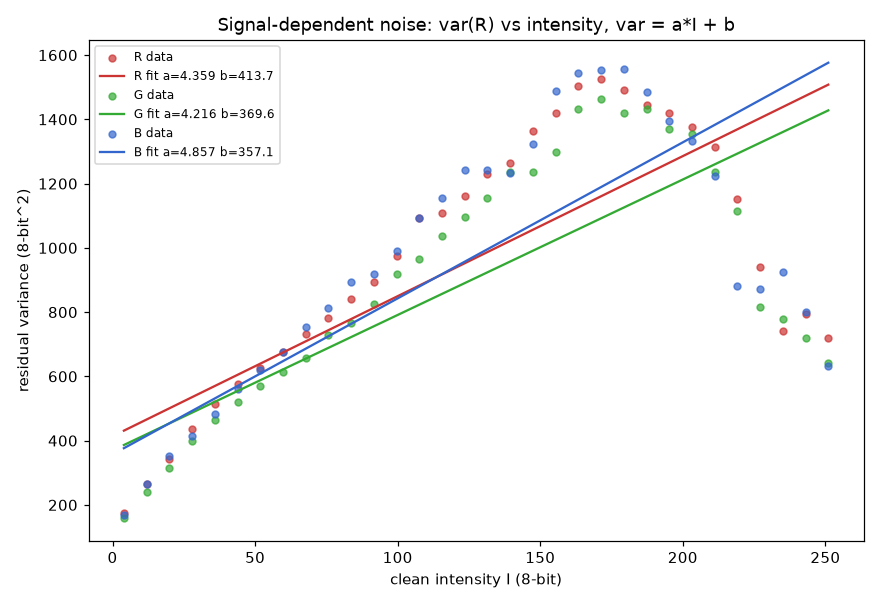
\includegraphics[width=\linewidth]{figs/fig2_variance_vs_intensity.png}
    \caption{Variance vs.\ intensity, fit $\mathrm{var}=aI+b$: slope is shot noise,
    intercept the read floor.}
    \label{fig:var}
  \end{subfigure}\hfill
  \begin{subfigure}{0.49\textwidth}
    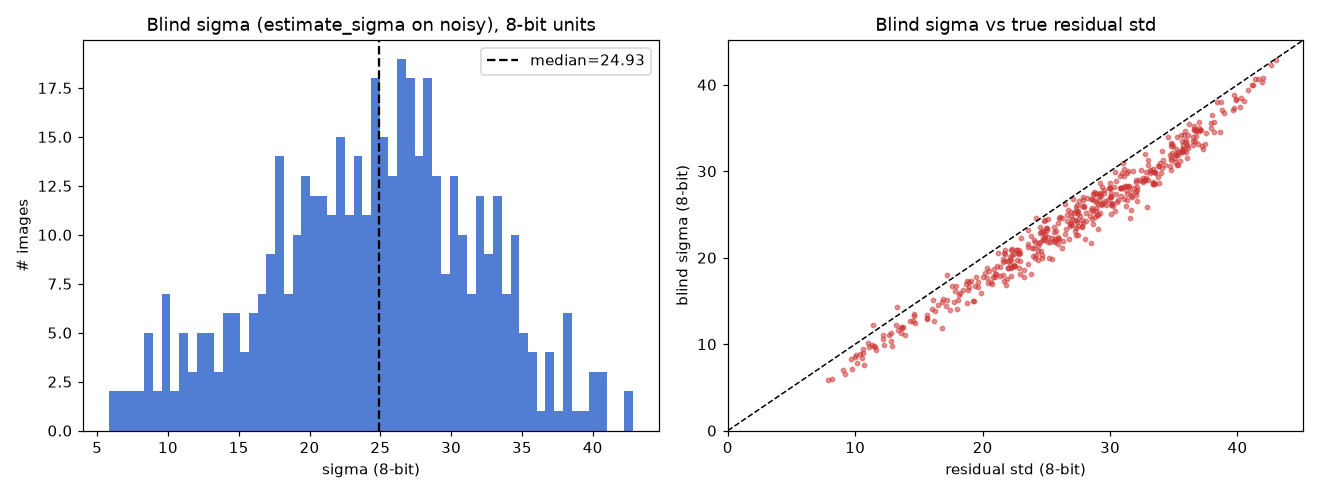
\includegraphics[width=\linewidth]{figs/fig3_sigma_distribution.png}
    \caption{Per-image blind $\sigma$, all 460 images: a continuum, no discrete levels.}
    \label{fig:sigma}
  \end{subfigure}
  \caption{The two measurements that most constrained the design.}
\end{figure}

\section{Solution architecture}

\begin{figure}[t]
\centering
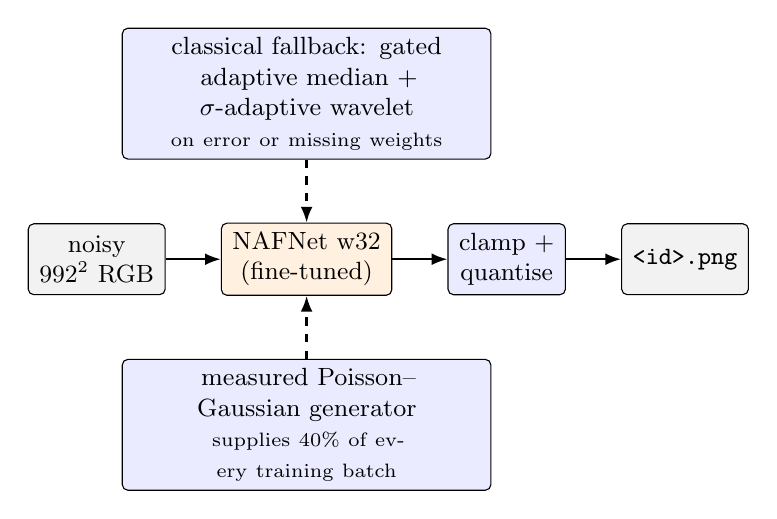
\begin{tikzpicture}[
  node distance=5mm and 7mm,
  box/.style={draw,rounded corners=2pt,align=center,minimum height=9mm,font=\small,inner xsep=4pt},
  cls/.style={box,fill=blue!8},
  net/.style={box,fill=orange!12},
  io/.style={box,fill=black!5},
  ar/.style={-{Latex[length=2mm]},thick}]
\node[io] (in) {noisy\\$992^2$ RGB};
\node[net,right=of in] (net) {NAFNet w32\\(fine-tuned)};
\node[cls,right=of net] (q) {clamp +\\quantise};
\node[io,right=of q] (out) {\texttt{<id>.png}};
\draw[ar] (in)--(net); \draw[ar] (net)--(q); \draw[ar] (q)--(out);
\node[cls,below=8mm of net,text width=44mm] (syn)
  {measured Poisson--Gaussian generator\\{\scriptsize supplies 40\% of every training batch}};
\draw[ar,dashed] (syn)--(net);
\node[cls,above=8mm of net,text width=44mm] (fb)
  {classical fallback: gated adaptive median $+$ $\sigma$-adaptive wavelet\\{\scriptsize on error or missing weights}};
\draw[ar,dashed] (fb)--(net);
\end{tikzpicture}
\caption{The pipeline. The scored path (solid) is deliberately minimal. The classical
components (blue, dashed) act \emph{around} it: the measured noise model synthesizes
40\% of the training data, and a complete classical denoiser stands by for any image the
network cannot process. There is a single implementation of the scored path
(\texttt{spcup/pipeline.py}), called by the submission entry point, the validator and the
ablation runner alike, so what we measure and what we submit cannot diverge.}
\label{fig:pipe}
\end{figure}

\paragraph{Stage 1 --- the measured noise model (classical), used to synthesize training data.}
This is where the classical signal processing does its real work. From the fits of \S2 we
built a generator reproducing the measured degradation, supplying $40\%$ of every
training batch from the training ground truths only. Two constraints make it faithful
rather than approximate, both caught by a verification script that compares synthesized
residuals against the measurements and refuses to proceed on a mismatch.

First, severity must satisfy $E[s^2]=1$: the fitted $a,b$ are pooled over the dataset and
so already average over severity, and our first attempt, $s\sim U(0.55,1.65)$ with
$E[s^2]=1.31$, inflated every synthetic variance by exactly that factor ($a,b$ came out
$17$--$36\%$ high). For $s\sim U(l,h)$ the constraint is $l^2+lh+h^2=3$. Second, the
measured excess kurtosis of $1.86$--$2.36$ cannot come from impulses alone ($0.033\%$ of
pixels is far too few) and must not come from inflating $\sigma$, which would break the
variance fit; we use a two-component Gaussian \emph{scale mixture} on the per-pixel
variance with weights solved so that $E[t]=1$ (variance exactly preserved) and
$E[t^2]=(K+3)/3$ for a target kurtosis $K$. The generator matches the measurement to
$2.5$--$13\%$ on $a,b$ and $7$--$10\%$ on kurtosis.

\paragraph{Stage 2 --- NAFNet restoration core (learned).}
NAFNet (width 32, encoder blocks $[2,2,4,8]$, 12 middle, decoder $[2,2,2,2]$;
29{,}159{,}715 parameters) predicts a residual that is added to the input. It was chosen
for quality per FLOP: the runtime component of the grade and the live final round both
reward a network that is practical on a CPU, and NAFNet's activation-free design
(SimpleGate plus simplified channel attention) matches transformer accuracy at a
fraction of the cost.

\paragraph{Stage 3 --- inference engineering.}
Since $992=2^5\times31$ is a multiple of 32, a four-level U-Net needs \emph{zero} padding
at full resolution, and the measured peak working set is 1.28\,GB, so we run the whole
image in one pass; tiling costs $3.5\times$ the runtime for no gain. Overlap-add tiling
with a raised-cosine partition of unity is retained only as an automatic out-of-memory
ladder ($\text{whole}\to512\to256\to\text{classical}$), alongside per-image exception
handling, so no input can make the run fail --- a crash forfeits the whole image score.
The tiled path agrees with the whole-image path to 45--50\,dB, with interior differences
of 6--10 levels confirming the blending is seam-free.

We also implemented TLC, the standard remedy for the statistics shift a globally-pooling
attention suffers when trained at $256^2$ and run at $992^2$, and measured three kernel
sizes; all were slightly \emph{worse} than leaving it off, because our checkpoints are
selected on full-resolution validation and so already account for the shift.

\section{Justification}

Every component is present, or absent, because a measurement supports it. The blind
design follows from finding (2); the absence of chroma processing from (5); the absence
of brightening from the residual mean. Three choices deserve explicit argument.

\textbf{Why the classical impulse filter is not in the network path.} Our
$\sigma(I)$-gated adaptive median --- which fixes a real defect in the baseline's
\emph{fixed} $64/255$ threshold, about $10\sigma$ on the cleanest images and
$\approx1.5\sigma$ on the noisiest --- is worth $+0.0152$ composite in the classical
pipeline. In front of the trained network it instead costs score, and a gate sweep shows
why: the composite rises monotonically as fewer pixels are filtered
($k=4.5\to0.5664$, $6\to0.5671$, $8\to0.5687$, $12\to0.5753$, off $\to0.5762$). That
dose--response curve is not a tuning miss. The network trains on impulses and hot pixels
injected by the generator, so it learns to repair them, and its prior beats a median. We
ship it where it helps (the fallback) and disable it where it does not.

\textbf{Why fine-tune rather than train from scratch.} We measured training throughput
on the available GPU (RTX 4050, 6\,GB) as pixel-bound at $\approx0.9$\,Mpx/s however
batch and patch are arranged. A twelve-hour budget is thus $\approx38{,}900$\,Mpx,
against the $838{,}000$\,Mpx of NAFNet's published SIDD schedule --- about $4.6\%$ of
the original training compute. Because the corruption is synthetic and we fitted its
generator, training \emph{data} is effectively free; the binding constraint is compute,
and a pretrained initialisation is the only thing that buys it. Starting from the
released SIDD weights (verified by exact file size, parameter count and a
\texttt{strict=True} load) the model scores \ZeroShotComp{} \emph{before any training},
already above the \BaseComp{} baseline.

\textbf{Why test-time augmentation is off by default.} An 8$\times$ $D_4$ self-ensemble
is worth about $+0.010$ composite, which at the 35\% weight of the image score is
$\approx+0.35\%$ of the final grade --- in exchange for a measured 7.6$\times$ the CPU
runtime, against a criterion worth 15\%. We measured the trade rather than assuming it
and ship with \texttt{--tta 1}; the option remains available and its effect is reported
in Table~\ref{tab:abl}.

\section{Alternatives considered}

Table~\ref{tab:alt} lists what we tested and rejected. Several are techniques the
low-light denoising literature would recommend by default and that this dataset
specifically does not support, so the negative results are as informative as the
positive ones.

\begin{table}[t]\centering\small
\begin{tabular}{p{44mm}p{68mm}r}
\toprule
Alternative & Why rejected & $\Delta$comp. \\
\midrule
Chroma smoothing & Measured $Cb/Y=0.84$, $Cr/Y=0.92$: chroma is quieter than luma here & Tab.~\ref{tab:abl} \\
Brightening / gamma & No exposure gap (residual mean $+1.5/255$) & Tab.~\ref{tab:abl} \\
Anscombe VST before net & Train/test mismatch; net trains on the raw distribution & Tab.~\ref{tab:abl} \\
Gated median before net & Dose--response sweep: helps the classical path, costs score here (\S4) & Tab.~\ref{tab:abl} \\
TLC local pooling & Checkpoints already selected at full resolution & $-0.004$ \\
SCUNet zero-shot & CPU-unfriendly; different degradation family & fallback \\
Training from scratch & Only $4.6\%$ of the reference compute is affordable (\S4) & not run \\
Hardcoded defect map & A dataset-derived lookup, not a generalisable procedure & by rule \\
\bottomrule
\end{tabular}
\caption{Alternatives considered and the evidence against each.}
\label{tab:alt}
\end{table}

\section{Methodology and validation strategy}

\textbf{Split.} The 460 public ids are sorted by the pre-computed blind $\sigma$ and
every 10th starting at index 5 is held out, giving \textbf{414 training / 46 validation}
images (every second validation image, 23 in total, forms a fast subset used during
training). The procedure is deterministic --- no random seed is involved --- and
severity-stratified by construction: the held-out $\sigma$ range is 7.57--40.66 against
5.86--42.83 for the full set. It is stored once and read by every script, so training,
validation and ablation cannot silently disagree about which images are held out. The
preliminary images 461--480 are never used for any tuning decision.

\textbf{Training data.} Batches mix real pairs with synthetic ones ($p=0.4$) built by the
generator of \S3 from the \emph{training} ground truths only, adding $0.033\%$ random
impulses and the 492 fixed hot pixels. Real pairs stay in the majority because the
generator only approximates those defect statistics. Augmentation is the dihedral group
(flips and $90^\circ$ rotations) and nothing photometric: the noise is
intensity-dependent, so any brightness or gamma jitter would place the image on a
different point of the $aI+b$ curve than the noise it carries.

\textbf{Objective.} We minimise \texttt{PSNRLoss}, the per-image log-MSE. This is a
correctness argument, not a preference: the competition metric averages \emph{per-image}
PSNR, whereas an $L_1$ or $L_2$ loss weights images by absolute error and lets the
noisiest dominate the gradient without earning proportionate credit. Optimiser AdamW
($\beta=(0.9,0.9)$, weight decay $10^{-3}$), learning rate $2\times10^{-4}$ with 500
warm-up steps and cosine decay to $10^{-6}$, fp16 mixed precision, gradient clipping at
1.0, and an exponential moving average (decay 0.9995) of the weights, which is evaluated
alongside the raw weights.

\textbf{Selection and scoring.} Checkpoints are selected on the \emph{validation
composite}, never on the loss, and predictions are quantised to 8-bit before scoring
because that is how they ship. All reported numbers come from the unmodified
\texttt{evaluation/evaluate.py}, used both as a subprocess and imported for per-image
rows, with the two cross-checked to $10^{-8}$ on every run. The torch metrics used for
in-training selection are separately asserted against scikit-image to better than
$2\times10^{-7}$.

\section{Results}

\begin{table}[t]\centering\small
\begin{tabular}{lrrrrr}
\toprule
Configuration & PSNR & SSIM & $\Delta$PSNR & Composite & s/img \\
\midrule
Noisy input (identity) & \NoisyPSNR & \NoisySSIM & 0.00 & 0.0000 & --- \\
Organizer baseline (median + NLM) & \BasePSNR & \BaseSSIM & $+4.51$ & \BaseComp & 0.97 \\
Pretrained NAFNet, zero-shot & 24.80 & 0.7996 & $+4.98$ & \ZeroShotComp & 9.8 \\
Classical only (no model) & 26.12 & 0.7580 & $+6.30$ & \ClassicalComp & 0.61 \\
\textbf{Ours (submitted)} & \textbf{\OursPSNR} & \textbf{\OursSSIM} & $\mathbf{+11.81}$ & \textbf{\OursComp} & \OursMs \\
\bottomrule
\end{tabular}
\caption{Held-out validation results (46 images), official metric.}
\label{tab:main}
\end{table}

\begin{table}[t]\centering\small
% Generated by: python scripts/tools/ablate.py --emit latex
\begin{tabular}{lrrr}
\toprule
Configuration & PSNR & SSIM & Composite \\
\midrule
Classical, no impulse pre-pass & 25.81 & 0.7509 & 0.3578 \\
Classical only (VST + wavelet + median) & 26.12 & 0.7580 & 0.3730 \\
\textbf{NAFNet, fine-tuned (submitted)} & \textbf{31.63} & \textbf{0.9195} & \textbf{0.6433} \\
Ours + TTA x4 & 31.69 & 0.9203 & 0.6456 \\
Ours + TTA x8 & 31.71 & 0.9207 & 0.6464 \\
Ours, tiled 512 (identity check) & 31.47 & 0.9194 & 0.6393 \\
\midrule
Ours + gated adaptive median pre-pass (rejected) & 31.32 & 0.9162 & 0.6304 \\
Ours + TLC(384) & 31.58 & 0.9193 & 0.6420 \\
Ours + chroma smoothing (rejected) & 31.60 & 0.9194 & 0.6421 \\
Ours + gamma 1.05 brightening (rejected) & 30.30 & 0.9167 & 0.6001 \\
Ours + Anscombe VST before net (rejected) & 29.51 & 0.9001 & 0.5655 \\
Classical with Anscombe VST (rejected variant) & 23.86 & 0.6848 & 0.2605 \\
\bottomrule
\end{tabular}

\caption{Ablation over the same 46 held-out images. Rows below the rule are
configurations we rejected; each was measured rather than argued away.}
\label{tab:abl}
\end{table}

\begin{figure}[t]
  \centering
  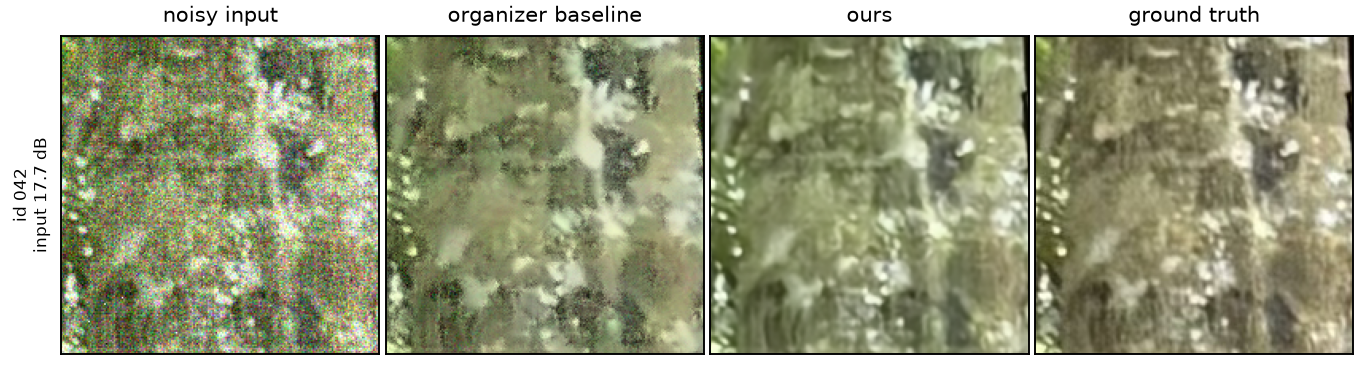
\includegraphics[width=0.92\textwidth]{figs/crops.png}
  \caption{The hardest held-out image by input noise level (centre crop, identical
  location in every panel). Detail and colour are recovered at the original brightness;
  no tone adjustment is applied anywhere.}
  \label{fig:crops}
\end{figure}

\section{Reproducibility and submission}

The pipeline contains no randomness at inference, so reproduction does not depend on
seeding (seeds and deterministic flags are set regardless). The default device is CPU
and the submitted images were generated on CPU, so the documented command reproduces
the submission on any machine. Outputs are quantised with $\lfloor 255x+0.5\rfloor$
(not banker's rounding) and written with fixed PNG encoder settings, so the file bytes
reproduce, not merely the pixels.

A preflight validator enforces every submission rule mechanically, including two
positive tests: the pipeline is re-run in a clean subprocess and compared by SHA-256
against the submitted files, and a \textbf{rename test} copies
\texttt{461\_noise.png} to \texttt{999\_noise.png} and asserts a byte-identical output
to \texttt{461.png} --- which no per-image lookup could satisfy.

\vspace{4pt}
\noindent\footnotesize
Code: \texttt{scripts/}. Entry point:
\texttt{python scripts/denoise.py --noise\_dir <in> --denoised\_dir <out>}
(\texttt{--input\_dir}/\texttt{--output\_dir} are accepted as aliases).
Commit SHA and model SHA-256 are recorded in \texttt{scripts/README.md}.

\end{document}